\documentclass{article}

\usepackage{graphicx}
\usepackage{tikz}
\usepackage{tikzsymbols}
\usetikzlibrary{calc,patterns,shapes.geometric}
\pagestyle{empty}
\usepackage[margin=0pt]{geometry}
\geometry{papersize={14in,12in}}

\def\centerarc[#1](#2)(#3:#4:#5){\draw[#1] ($(#2)+({#5*cos(#3)},{#5*sin(#3)})$) arc (#3:#4:#5);}

\begin{document}
	\begin{figure}
		\centering
		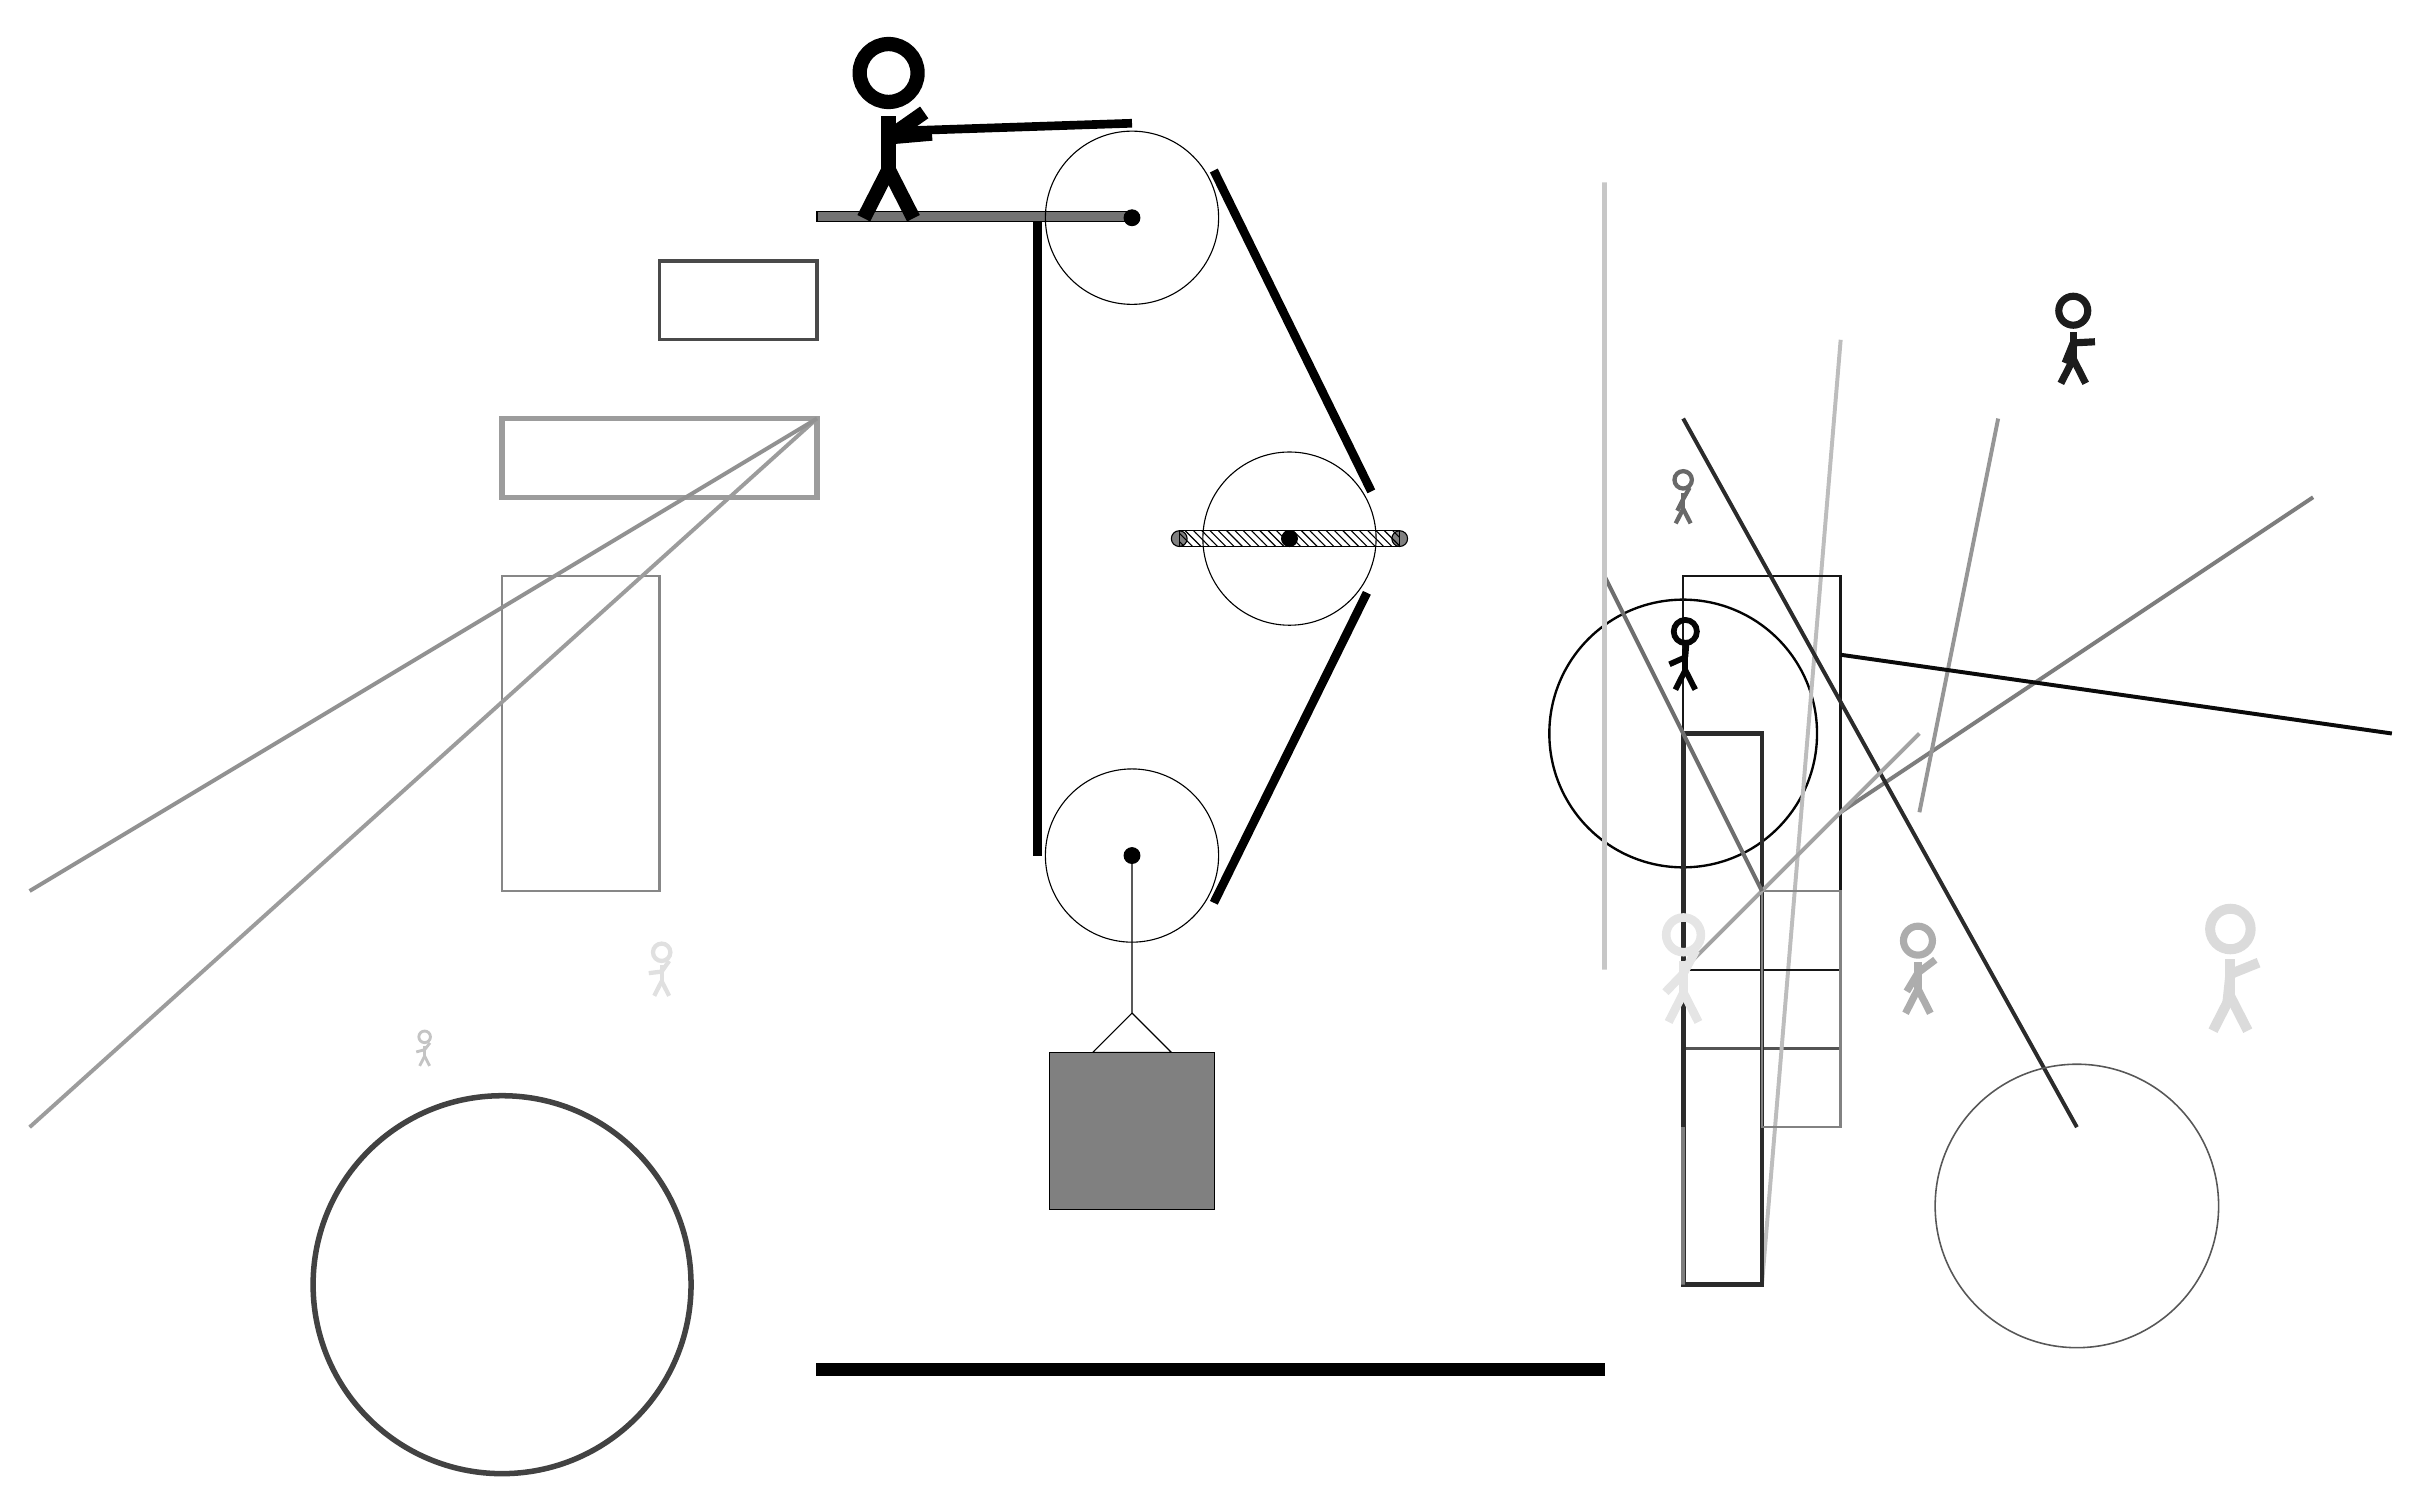
\begin{tikzpicture}
			%%%%% START %%%%%
			
			\draw[fill=black!55] (-2, 11.5) rectangle (2, 11.625);
			
			\draw (2, 3.45) circle (1.1);
			\draw[fill=black] (2, 3.45) circle (0.1);
			
			\draw (2, 11.55) circle (1.1);
			\draw[fill=black] (2, 11.55) circle (0.1);
			
			\draw[fill=white](4, 7.475) circle (1.1);
			\draw[fill=black] (4, 7.475) circle (0.1);
			\draw[fill=black!50] (2.6, 7.475) circle (0.1);
			\draw[fill=black!50] (5.4, 7.475) circle (0.1);
			\draw[pattern=north west lines, pattern color=black] (2.6, 7.575) rectangle (5.4, 7.375);
			
			\draw (2, 3.45) -- (2, 1.45) -- (1.5, 0.95) -- (2.5, 0.95) -- (2, 1.45);
			\draw[fill=black!50] (0.95, 0.95) rectangle (3.05, -1.05);
			
			\draw[line width=0.4mm, color=black!71] (-4, 11) rectangle (-2, 10);
			
			\draw [line width=0.3mm, color=black!99](9, 5) circle (1.7);
			\draw[line width=0.5mm, color=black!51](11, 4) -- (17, 8);
			\node[line width=0.4mm, color=black!32] at (12, 2) {\Strichmaxerl[5][59][37]};
			
			\draw[line width=0.4mm, color=black!67] (9, 1) rectangle (11, 1);
			\node[line width=0.2mm, color=black!14] at (16, 2) {\Strichmaxerl[7][84][22]};
			\draw[line width=0.5mm, color=black!26](10, -2) -- (11, 10);
			
			\node[line width=0.5mm, color=black!12] at (-4, 2) {\Strichmaxerl[3][7][55]};
			\draw[line width=0.3mm, color=black!91] (9, 2) rectangle (11, 7);
			
			\draw[line width=0.7mm, color=black!39] (-2, 8) rectangle (-6, 9);
			\draw[line width=0.6mm, color=black!83] (10, -2) rectangle (9, 5);
			
			\draw[line width=0.5mm, color=black!41](12, 4) -- (13, 9);
			\draw [line width=0.7mm, color=black!74](-6, -2) circle (2.4);
			
			\draw[line width=0.3mm, color=black!47] (-4, 7) rectangle (-6, 3);
			\node[line width=0.5mm, color=black!23] at (-7, 1) {\Strichmaxerl[2][15][52]};
			\draw[line width=0.5mm, color=black!83](9, 9) -- (14, 0);
			
			\node[line width=0.2mm, color=black!98] at (9, 6) {\Strichmaxerl[4][24][85]};
			\node[line width=0.7mm, color=black!59] at (9, 8) {\Strichmaxerl[3][63][61]};
			\node[line width=0.4mm, color=black!89] at (14, 10) {\Strichmaxerl[5][68][3]};
			
			\draw[line width=0.5mm, color=black!39](-2, 9) -- (-12, 0);
			\draw [line width=0.2mm, color=black!66](14, -1) circle (1.8);
			
			\draw[line width=0.5mm, color=black!96](11, 6) -- (18, 5);
			
			\draw[line width=0.3mm, color=black!49] (10, 0) rectangle (11, 3);
			\draw[line width=0.5mm, color=black!36](9, 2) -- (12, 5);
			\draw[line width=0.5mm, color=black!51] (9, -2) rectangle (9, 0);
			\draw [line width=0.3mm, color=black!86](-7, 5) circle (0.0);
			
			\draw[line width=0.5mm, color=black!57](10, 3) -- (8, 7);
			\draw[line width=0.7mm, color=black!22] (8, 2) rectangle (8, 12);
			\draw[line width=0.5mm, color=black!43](-2, 9) -- (-12, 3);
			
			\node[line width=0.3mm, color=black!10] at (9, 2) {\Strichmaxerl[6][46][62]};
			
			\draw[line width=1.1mm] (0.8, 11.5) -- (0.8, 3.45);
			\centerarc[line width=1.1mm](2, 3.45)(180:330:1.2000000000000002);
			\draw[line width=1.1mm](3.0392, 2.85) -- (4.983, 6.7867);
			\centerarc[line width=1.1mm](4, 7.475)(390:325:1.2000000000000002);
			\draw[line width=1.1mm](5.0392, 8.075) -- (3.0392, 12.15);
			\centerarc[line width=1.1mm](2, 11.55)(30:90:1.2000000000000002);
			\draw[line width=1.1mm](2, 12.75) -- (-1, 12.65);
			
			\node at (-1, 12.65) {\Strichmaxerl[10][-175][35]};
			
			\draw[fill=black] (-2, -3) rectangle (8, -3.15);
			
			%%%%% END %%%%%
		\end{tikzpicture}
	\end{figure}	
\end{document}